\section{Design Flow}
\label{sec:designflow}

Based on the introduction and motivation we demonstrated above, we design our headroom experiments and online strategy as follows. 


\begin{figure}[ht!]
	\centering
	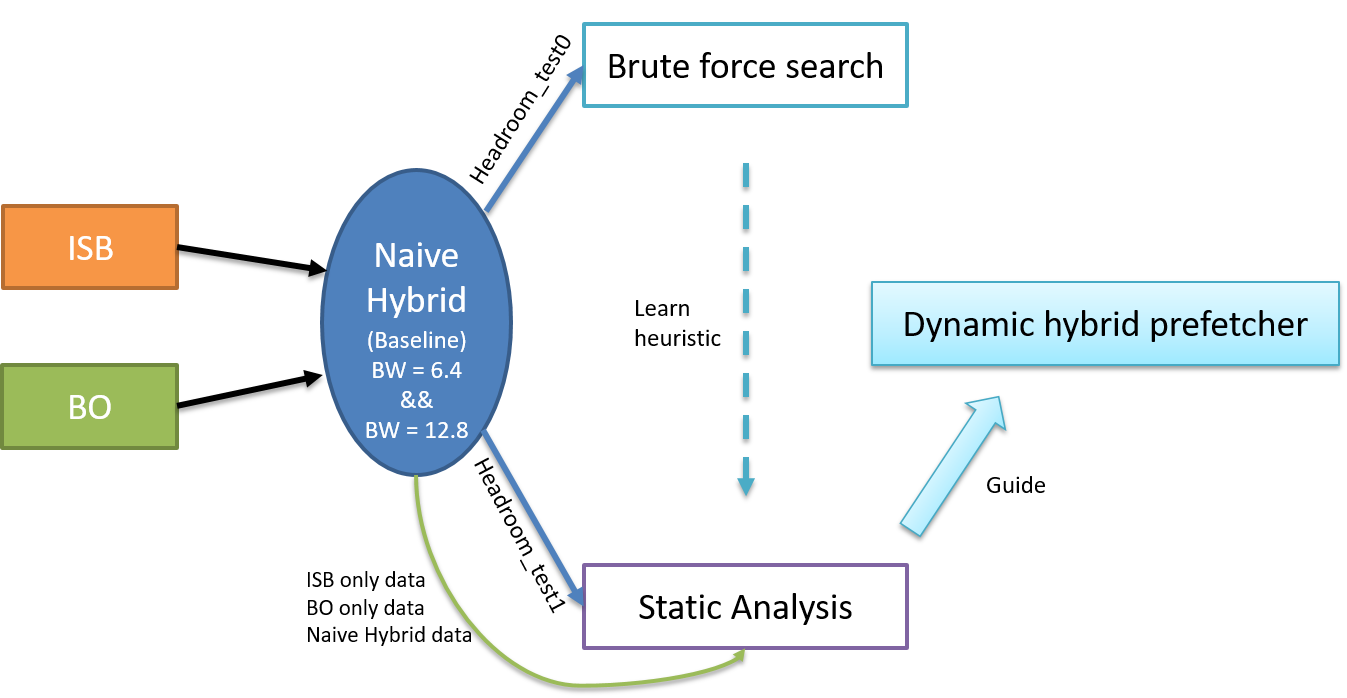
\includegraphics[width=1.0\textwidth]{images/design_flow.png}
	\caption{Design flow}
	\label{fig:design_flow}
\end{figure}

The Brute Force and Static Analysis are both offline headroom designs which will be described in the following two sections. Brute Force Search tries each choice on each PC, and finds out the best decisions and optimal headroom. Static Analysis comes up with a heuristic. It uses the statistics of each PC from ISB, BO and naive hybrid experiments as input, and builds a strategy that makes decisions closest to Brute Force Search thus achieves best speedup. Finally the Static Analysis guides the design of our dynamic hybrid system.


  \subsection{Brute Force Search}
  \label{sec:bruteforcesearch}
  
  Introduce how brute force search works \par
  In this part, we will first illustrate why we need a Brute Force Search to find the headroom of PC localization. Then we show how to Brute Force Search headroom experiment is designed. \par
  
  \subsubsection{Metric to measure a PC}
  \label{sec:metricPC}
  
  It is known that accuracy and coverage are two good metrics to measure a prefetcher. They are calculated as follows:
  \begin{equation}
 Accuracy = \frac{prefetch\ hits}{total\  prefetched} 
 \end{equation}
  \begin{equation}
  Coverage = \frac{prefetch\ hits}{prefetch\ hits + total\ misses}
  \end{equation}
  
  Similarly we can define accuracy and coverage of a trigger PC:
  \begin{equation}
  PC\ Accuracy = \frac{prefetch\ hits}{prefetched\ by\ this\ PC}
  \end{equation}
  \begin{equation}
  PC\ Coverage = \frac{prefetch\ hits}{prefetch\ hits + total\ misses}
 \end{equation}
 
 However, it turns out that these two metrics from ISB and BO can't determine the preference of a PC. 
 
 \begin{figure}[ht!]
	\centering
	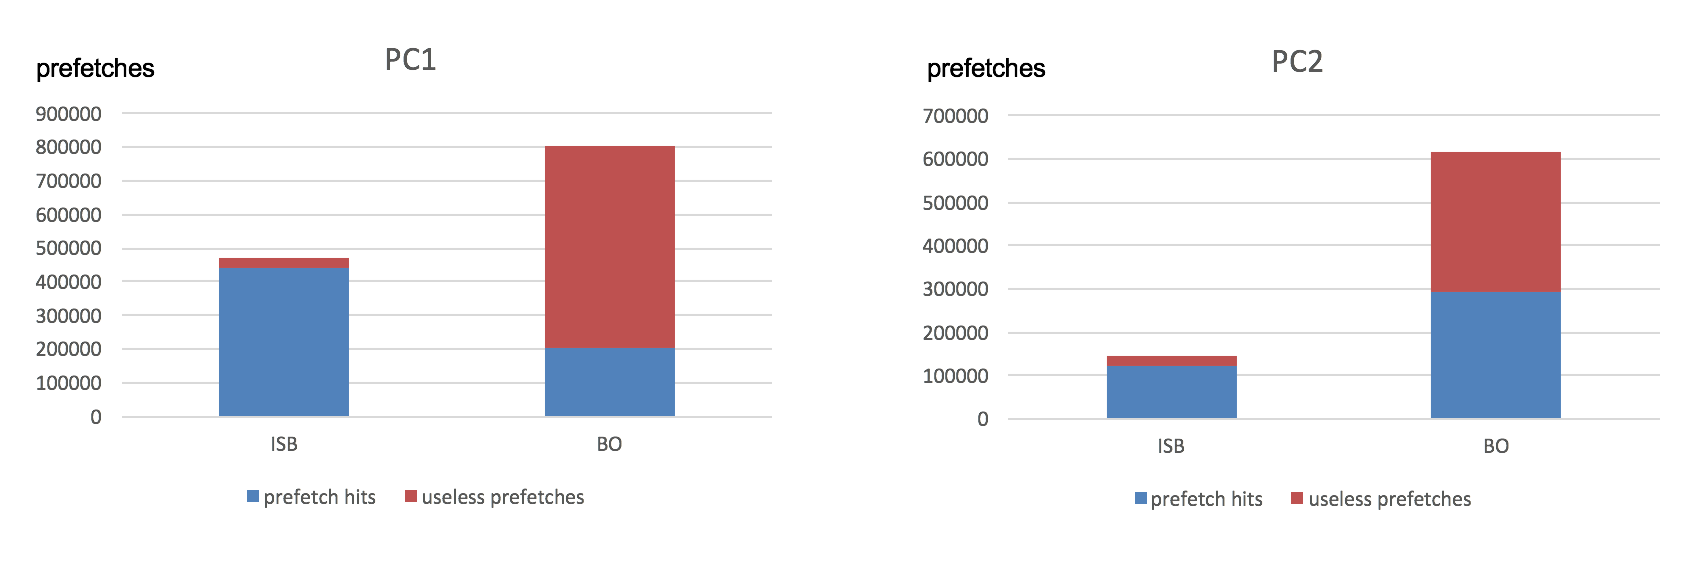
\includegraphics[width=1.0\textwidth]{images/metric.png}
	\caption{Hits and useless prefetches example}
	\label{fig:metric}
\end{figure}

For example in Fig.\ref{fig:metric}, on PC1, it is clear that ISB on this PC has higher accuracy and coverage, so the hybrid system should choose ISB. But on PC2, ISB has higher accuracy but BO has higher coverage, then it's hard to choose. In terms of speedup, prefetch hits has positive contribution and useless prefetches has negative contribution. On PC2, BO has more prefetch hits and more useless prefetches, so it's hard to infer its contribution is positive or negative only on this numbers. 
  
    \subsubsection{Design of Brute Force Search}
  \label{sec:designBFS}
  Since the effect of accuracy and coverage of a PC to the overall performance is not clear, we design the Brute Force Search experiment to explore the space of PC's choices and find out the headroom. \par
  The steps are: \par
  1) Choose several PCs with most prefetches. For each pinpoint, we find out the PC with most prefetches MAX. Any PCs that has prefetches more than 5\% of MAX are chosen.\par 
  2) Find the best decision of each PC. For each PC, run four experiments, respectively set its decision to ISB, BO, neither or both. \textbf{All other PCs are set to choose both}.\par
  3) Combine the best decisions of all PCs.\par
  Note that for the several PCs we consider, they can cover more than 95\% of total prefetches, so they are representative enough to the performance. \par
  Here the Brute Force Search design is not optimal. An optimal exploration should run all the possible choices over all PCs, i.e. $4^{n}$ experiments, n is the number of PC considered, which it is around 10 to 30. 
  This exploration space is too large and needs too many experiments, so we take one step back and design this suboptimal search, which need 4*n experiments. Because it sets all non-considered PC to both, it's basically compare the four choices to all PCs choosing both, which might over estimate the bandwidth consumption. \par
  
  
  
  \subsection{Static Analysis}
  \label{sec:staticanalysis}


 